% [ignoring loop detection]
\documentclass[12pt]{article}

\usepackage[a4paper, margin=1in]{geometry}
\usepackage{tikz}
\usepackage{amsmath}
\usetikzlibrary{shapes.geometric, shapes.misc, arrows.meta, positioning, shadows, backgrounds, fit, calc}

% --- Global TikZ Styles ---
\tikzset{
    base/.style = {
        draw=black, very thick, text centered, 
        minimum height=3.5em, drop shadow, font=\sffamily\small
    },
    % Components
    process/.style = {base, rectangle, rounded corners, fill=blue!10, text width=9em},
    hw/.style      = {base, rectangle, rounded corners, fill=green!10, text width=9em},
    cloud/.style   = {base, ellipse, fill=cyan!10, text width=8em},
    ai/.style      = {base, rectangle, rounded corners, fill=purple!10, text width=10em},
    data/.style    = {base, cylinder, fill=yellow!10, shape border rotate=90, aspect=0.25, text width=6em, minimum height=4em},
    startend/.style= {base, rounded rectangle, fill=gray!20, text width=7em},
    % Edges and annotations
    arrow/.style = {thick, ->, >=Stealth},
    dashed_arrow/.style = {thick, dashed, ->, >=Stealth},
    annotation/.style = {font=\scriptsize\sffamily, text=black!70, align=center}
}

\title{\textbf{IoT Virtual Lab}\\System Architecture \& Informatic Diagrams}
\author{}
\date{}

\begin{document}

\maketitle

\section*{1. Firmware Sensor Polling Strategy (Mega2560)}
\textit{This flowchart details the embedded C++ execution loop, explicitly showing the non-blocking multi-rate hardware polling and data serialization.}
\begin{figure}[h]
\centering
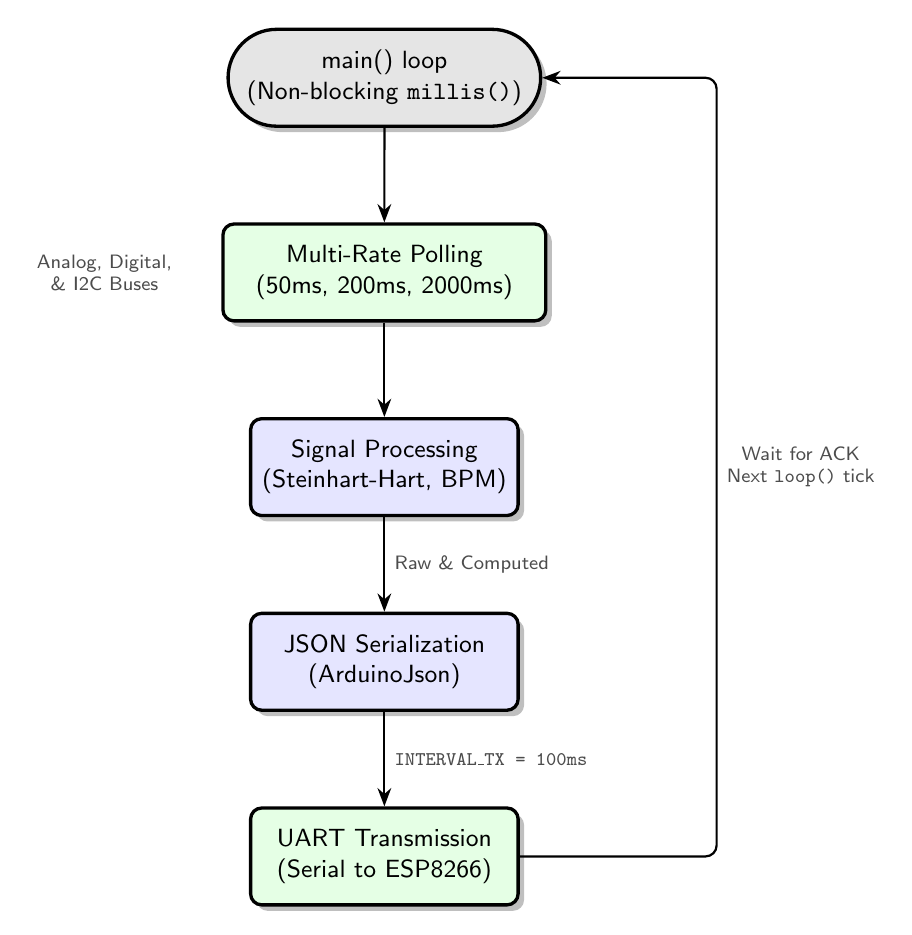
\begin{tikzpicture}[node distance=1.2cm and 2cm]
    \node (start) [startend, text width=10em] {main() loop\\(Non-blocking \texttt{millis()})};
    
    \node (analog) [hw, below=of start, text width=11em] {Multi-Rate Polling\\(50ms, 200ms, 2000ms)};
    \node (adc) [annotation, left=0.5cm of analog] {Analog, Digital,\\\& I2C Buses};
    
    \node (process) [process, below=of analog] {Signal Processing\\(Steinhart-Hart, BPM)};
    \node (json) [process, below=of process] {JSON Serialization\\(ArduinoJson)};
    \node (send) [hw, below=of json] {UART Transmission\\(Serial to ESP8266)};

    \draw [arrow] (start) -- (analog);
    \draw [arrow] (analog) -- (process);
    \draw [arrow] (process) -- node[right, annotation] {Raw \& Computed} (json);
    \draw [arrow] (json) -- node[right, annotation] {\texttt{INTERVAL\_TX = 100ms}} (send);
    
    % Feedback loop
    \draw [arrow, rounded corners] (send.east) -- ++(2.5,0) |- node[pos=0.25, right, annotation] {Wait for ACK\\Next \texttt{loop()} tick} (start.east);
\end{tikzpicture}
\end{figure}

\newpage

\section*{2. Backend Hybrid Mode Architecture}
\textit{This diagram highlights the dual-ingestion capability of the Node.js backend, merging physical IoT data with simulated mock streams.}
\begin{figure}[h]
\centering
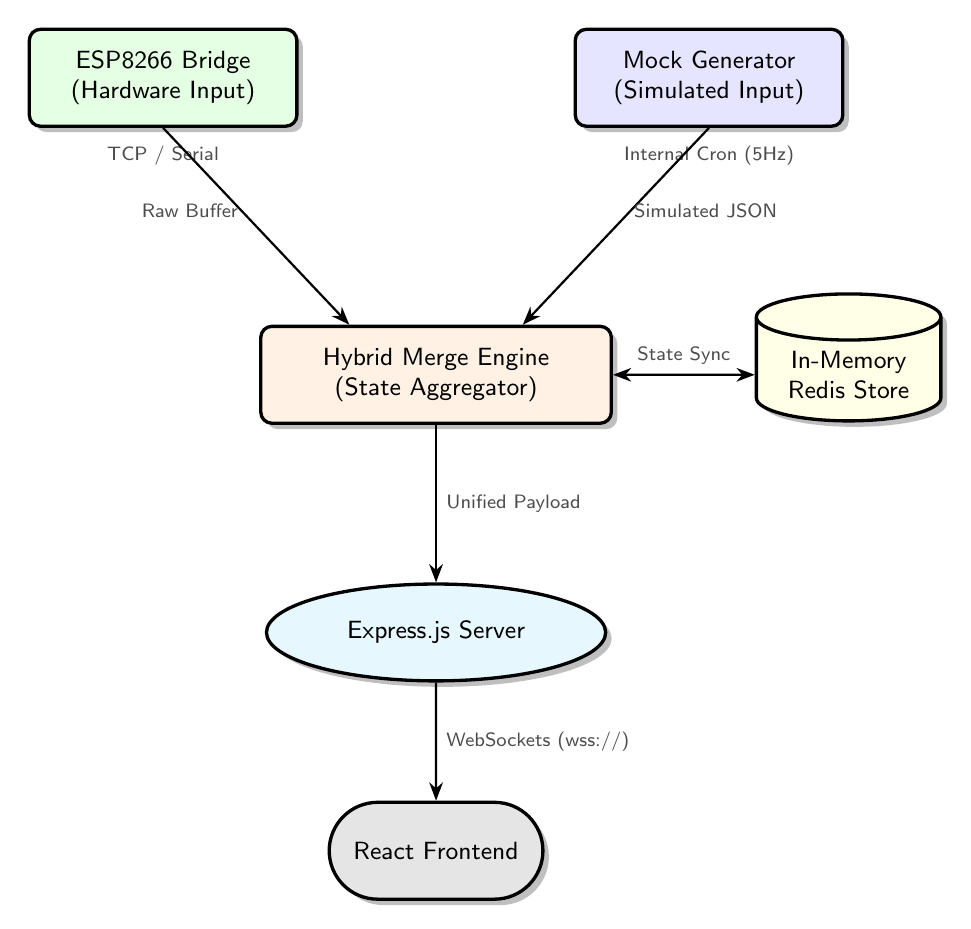
\begin{tikzpicture}[node distance=2.5cm and 1cm]
    % Central merge node
    \node (merge) [process, fill=orange!10, text width=12em] {Hybrid Merge Engine\\(State Aggregator)};
    
    % Position inputs above and to the sides
    \node (hw) [hw, above left=2.5cm and -0.5cm of merge] {ESP8266 Bridge\\(Hardware Input)};
    \node (mock) [process, above right=2.5cm and -0.5cm of merge] {Mock Generator\\(Simulated Input)};

    \node (tcp) [annotation, below=0.1cm of hw] {TCP / Serial};
    \node (internal) [annotation, below=0.1cm of mock] {Internal Cron (5Hz)};

    % Redis spaced out nicely to the right
    \node (db) [data, right=1.8cm of merge] {In-Memory\\Redis Store};
    
    \node (backend) [cloud, below=2cm of merge] {Express.js Server};
    \node (client) [startend, below=1.5cm of backend] {React Frontend};

    % Clean diagonal lines to the top edge of merge (angles 150 and 30)
    \draw [arrow] (hw.south) -- node[left, annotation, xshift=-0.1cm, yshift=0.2cm] {Raw Buffer} (merge.150);
    \draw [arrow] (mock.south) -- node[right, annotation, xshift=0.1cm, yshift=0.2cm] {Simulated JSON} (merge.30);
    
    \draw [arrow, <->] (merge) -- node[above, annotation] {State Sync} (db);
    \draw [arrow] (merge) -- node[right, annotation] {Unified Payload} (backend);
    \draw [arrow] (backend) -- node[right, annotation] {WebSockets (wss://)} (client);
\end{tikzpicture}
\end{figure}

\newpage

\section*{3. AI Context Injection Workflow (Gemini 2.5 Flash)}
\textit{This data flow pipeline demonstrates how live lab state is injected into the LLM system prompt to provide context-aware tutoring.}
\begin{figure}[h]
\centering
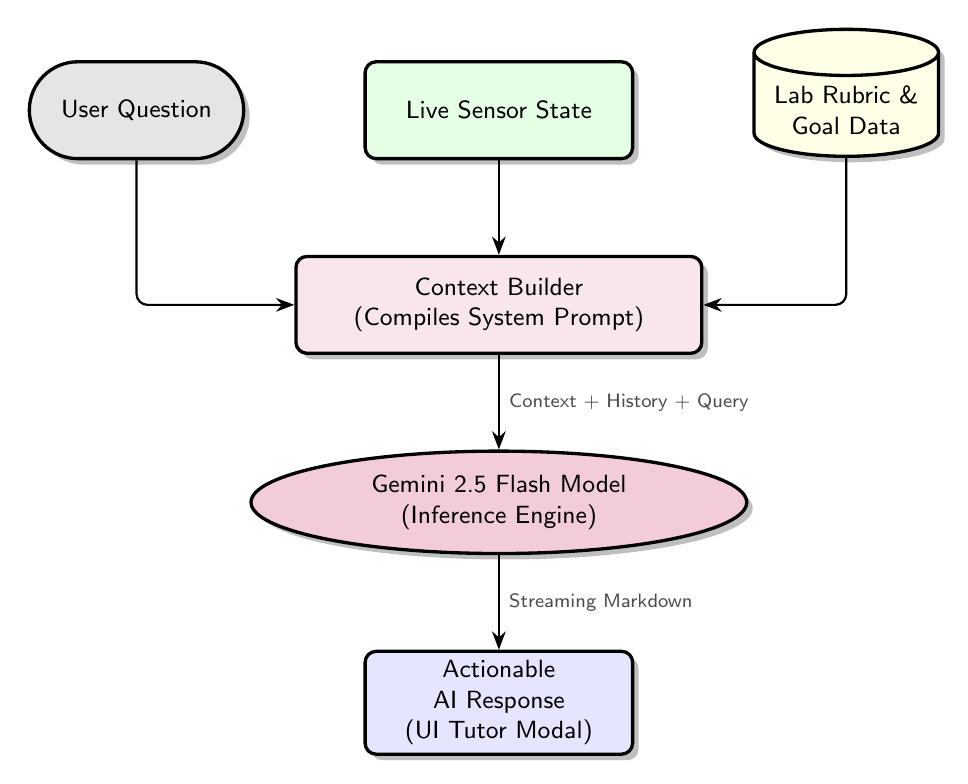
\begin{tikzpicture}[node distance=1.2cm and 1.5cm]
    \node (sensor) [hw] {Live Sensor State};
    \node (rubric) [data, right=of sensor] {Lab Rubric \&\\Goal Data};
    \node (user) [startend, left=of sensor] {User Question};

    \node (context) [ai, below=of sensor, text width=14em] {Context Builder\\(Compiles System Prompt)};
    
    \node (llm) [cloud, fill=purple!20, below=of context, text width=12em] {Gemini 2.5 Flash Model\\(Inference Engine)};
    \node (response) [process, below=of llm] {Actionable AI Response\\(UI Tutor Modal)};

    \draw [arrow] (sensor) -- (context);
    \draw [arrow, rounded corners] (rubric) |- (context);
    \draw [arrow, rounded corners] (user) |- (context);
    
    \draw [arrow] (context) -- node[right, annotation] {Context + History + Query} (llm);
    \draw [arrow] (llm) -- node[right, annotation] {Streaming Markdown} (response);
\end{tikzpicture}
\end{figure}

\newpage

\section*{4. DSP: Moving Average Filter}
\textit{This is a mathematical signal processing diagram illustrating the smoothing of noisy ADC readings.}
\begin{figure}[h]
\centering
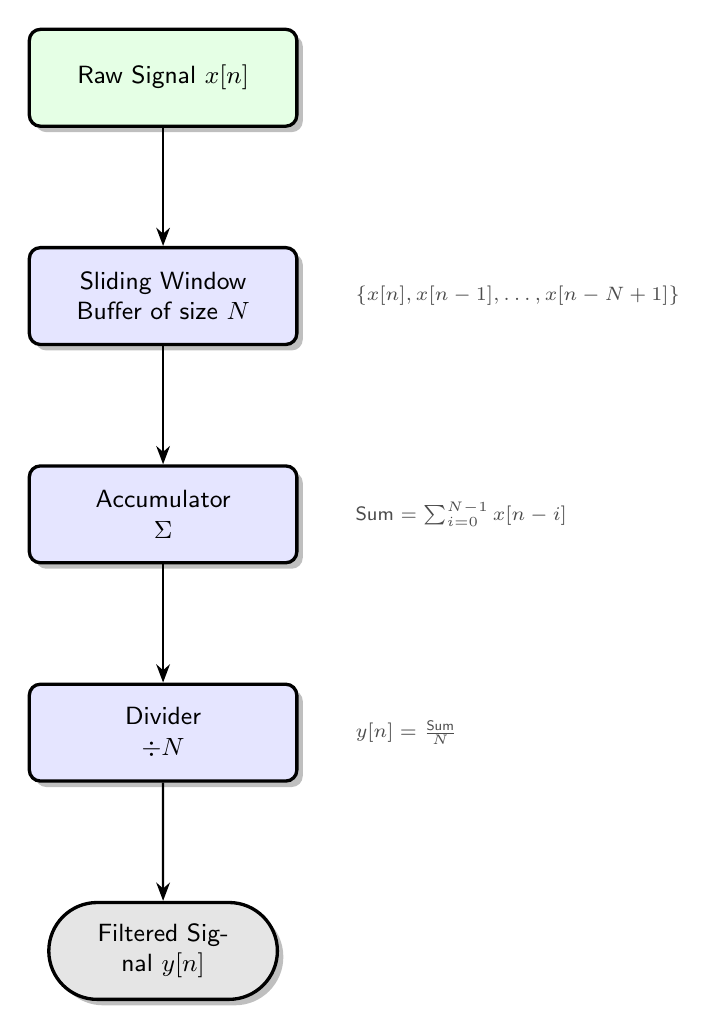
\begin{tikzpicture}[node distance=1.5cm]
    \node (input) [hw] {Raw Signal $x[n]$};
    
    \node (buffer) [process, below=of input] {Sliding Window\\Buffer of size $N$};
    \node (math1) [annotation, right=0.6cm of buffer] {$\{x[n], x[n-1], \dots, x[n-N+1]\}$};

    \node (sum) [process, below=of buffer] {Accumulator\\$\Sigma$};
    \node (math2) [annotation, right=0.6cm of sum] {Sum = $\sum_{i=0}^{N-1} x[n-i]$};

    \node (divide) [process, below=of sum] {Divider\\$\div N$};
    \node (math3) [annotation, right=0.6cm of divide] {$y[n] = \frac{\text{Sum}}{N}$};

    \node (output) [startend, below=of divide] {Filtered Signal $y[n]$};

    \draw [arrow] (input) -- (buffer);
    \draw [arrow] (buffer) -- (sum);
    \draw [arrow] (sum) -- (divide);
    \draw [arrow] (divide) -- (output);
\end{tikzpicture}
\end{figure}

\newpage

\section*{5. Deployment Infrastructure (Network Topology)}
\textit{This diagram maps the physical and cloud infrastructure boundaries, distinguishing between the local lab network and cloud deployments.}
\begin{figure}[h]
\centering
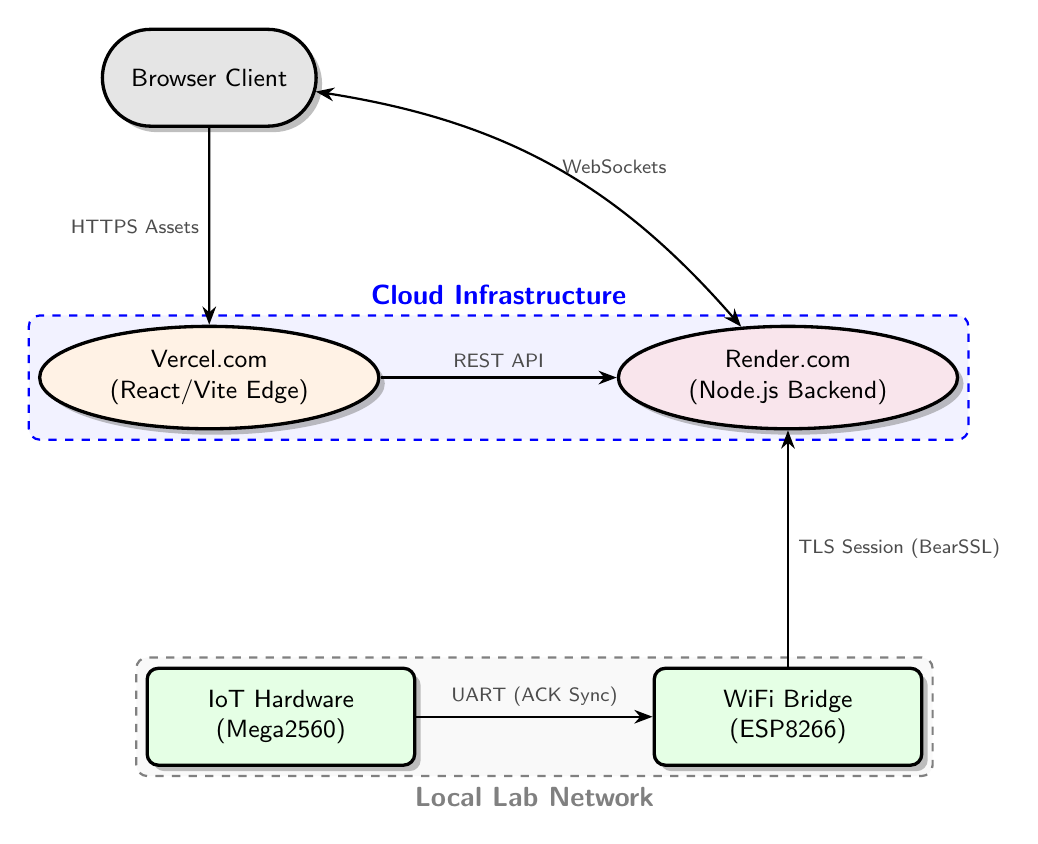
\begin{tikzpicture}[node distance=2cm and 3cm]
    
    % Nodes
    \node (iot) [hw] {IoT Hardware\\(Mega2560)};
    \node (bridge) [hw, right=of iot] {WiFi Bridge\\(ESP8266)};
    
    \node (backend) [cloud, fill=purple!10, above=3cm of bridge] {Render.com\\(Node.js Backend)};
    \node (frontend) [cloud, fill=orange!10, left=of backend] {Vercel.com\\(React/Vite Edge)};
    
    \node (user) [startend, above=2.5cm of frontend] {Browser Client};

    % Boundaries (Backgrounds)
    \begin{scope}[on background layer]
        \node [draw=gray, dashed, thick, rounded corners, fill=gray!5, fit=(iot) (bridge), label={[font=\sffamily\bfseries, gray]below:Local Lab Network}] {};
        
        \node [draw=blue, dashed, thick, rounded corners, fill=blue!5, fit=(backend) (frontend), label={[font=\sffamily\bfseries, blue]above:Cloud Infrastructure}] {};
    \end{scope}

    % Edges
    \draw [arrow] (iot) -- node[above, annotation] {UART (ACK Sync)} (bridge);
    \draw [arrow] (bridge) -- node[right, annotation] {TLS Session (BearSSL)} (backend);
    
    \draw [arrow] (frontend) -- node[above, annotation] {REST API} (backend);
    \draw [arrow, <->] (backend) edge[bend right=20] node[right, annotation] {WebSockets} (user);
    
    \draw [arrow] (user) -- node[left, annotation] {HTTPS Assets} (frontend);
\end{tikzpicture}
\end{figure}

\newpage

\section*{6. Latency \& Concurrency Timeline}
\textit{This timeline explicitly compares the real-time sensor transmission loop (200ms) against the asynchronous AI inference (3-5s).}
\begin{figure}[h]
\centering
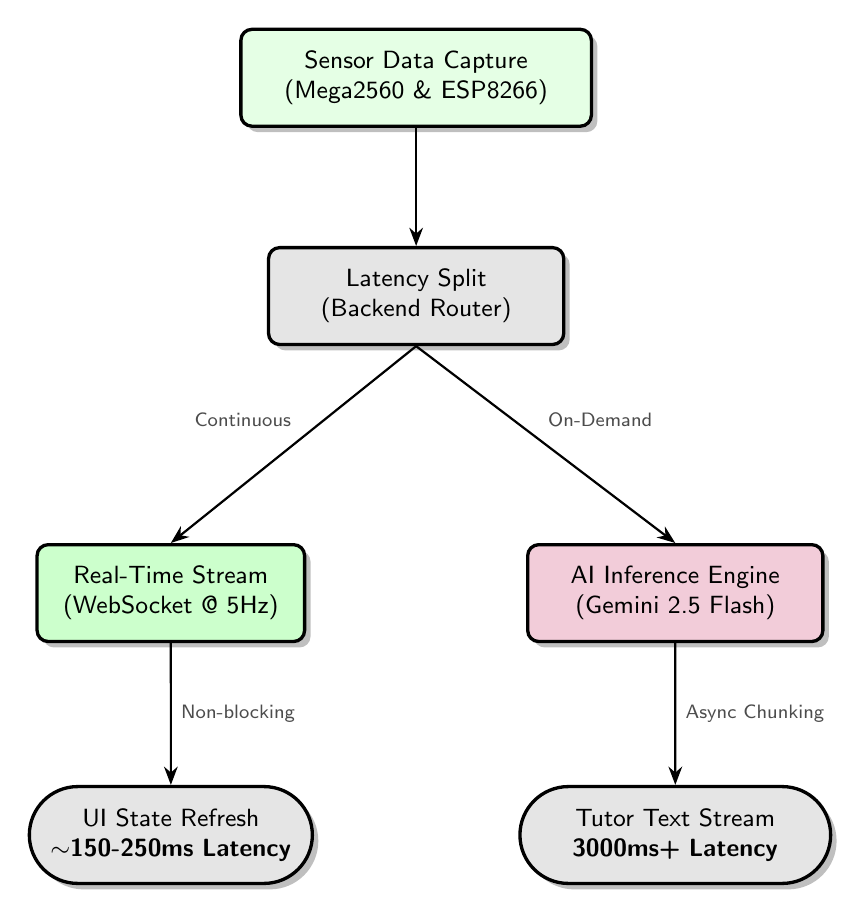
\begin{tikzpicture}[node distance=2.5cm and 1cm]
    \node (input) [hw, text width=12em] {Sensor Data Capture\\(Mega2560 \& ESP8266)};
    
    \node (split) [process, below=1.5cm of input, fill=gray!20, text width=10em] {Latency Split\\(Backend Router)};

    \node (fast) [hw, below left=2.5cm and -0.5cm of split, fill=green!20] {Real-Time Stream\\(WebSocket @ 5Hz)};
    \node (slow) [ai, below right=2.5cm and -0.5cm of split, fill=purple!20] {AI Inference Engine\\(Gemini 2.5 Flash)};

    \node (ui) [startend, below=1.8cm of fast, text width=9em] {UI State Refresh\\\textbf{$\sim$150-250ms Latency}};
    \node (airesp) [startend, below=1.8cm of slow, text width=10em] {Tutor Text Stream\\\textbf{3000ms+ Latency}};

    \draw [arrow] (input) -- (split);
    % Clean diagonal lines to the top edge of fast and slow
    \draw [arrow] (split.south) -- node[above left, annotation, xshift=0.1cm, yshift=0.1cm] {Continuous} (fast.north);
    \draw [arrow] (split.south) -- node[above right, annotation, xshift=-0.1cm, yshift=0.1cm] {On-Demand} (slow.north);
    
    \draw [arrow] (fast) -- node[right, annotation] {Non-blocking} (ui);
    \draw [arrow] (slow) -- node[right, annotation] {Async Chunking} (airesp);
\end{tikzpicture}
\end{figure}
\newpage

\section*{7. Frontend Application Architecture}
\textit{This block diagram maps the component structure of the React frontend, showing how real-time hooks and AI contexts feed into the UI layers.}
\begin{figure}[h]
\centering
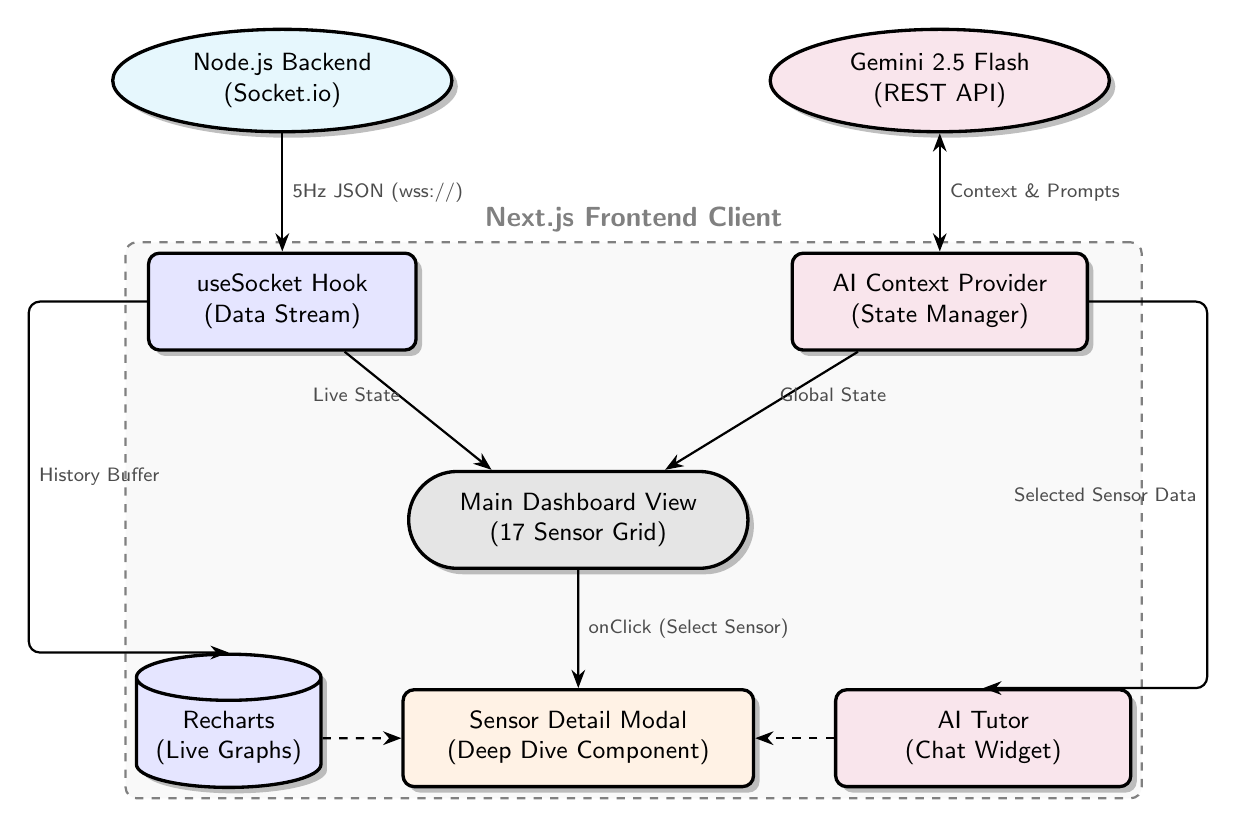
\begin{tikzpicture}[node distance=2cm and 1.5cm]
    
    % External Sources (Top Row)
    \node (backend) [cloud, fill=cyan!10] {Node.js Backend\\(Socket.io)};
    \node (llm) [cloud, fill=purple!10, right=4cm of backend] {Gemini 2.5 Flash\\(REST API)};

    % State & Hooks Layer
    \node (socket_hook) [process, below=1.5cm of backend] {useSocket Hook\\(Data Stream)};
    \node (ai_context) [ai, below=1.5cm of llm] {AI Context Provider\\(State Manager)};

    % UI Layer - Dashboard
    \node (dashboard) [startend, below right=1.5cm and 0.5cm of socket_hook, text width=11em] {Main Dashboard View\\(17 Sensor Grid)};
    
    % UI Layer - Detail Modal
    \node (modal) [process, below=1.5cm of dashboard, text width=12em, fill=orange!10] {Sensor Detail Modal\\(Deep Dive Component)};

    % Sub-components for the Modal
    \node (charts) [data, left=1cm of modal, fill=blue!10] {Recharts\\(Live Graphs)};
    \node (tutor) [ai, right=1cm of modal, fill=purple!10] {AI Tutor\\(Chat Widget)};

    % --- Connections ---
    
    % External to Hooks
    \draw [arrow] (backend) -- node[right, annotation] {5Hz JSON (wss://)} (socket_hook);
    \draw [arrow, <->] (llm) -- node[right, annotation] {Context \& Prompts} (ai_context);
    
    % Hooks to Dashboard
    \draw [arrow] (socket_hook) -- node[left, annotation, xshift=-0.1cm, yshift=0.2cm] {Live State} (dashboard.150);
    \draw [arrow] (ai_context) -- node[right, annotation, xshift=0.1cm, yshift=0.2cm] {Global State} (dashboard.30);

    % Dashboard to Modal
    \draw [arrow] (dashboard) -- node[right, annotation] {onClick (Select Sensor)} (modal);
    
    % Hooks to Sub-components
    % Route socket hook down to charts
    \draw [arrow, rounded corners] (socket_hook.west) -- ++(-1.5,0) |- node[pos=0.25, right, annotation] {History Buffer} (charts.north);
    % Route AI context down to tutor
    \draw [arrow, rounded corners] (ai_context.east) -- ++(1.5,0) |- node[pos=0.25, left, annotation] {Selected Sensor Data} (tutor.north);

    % Sub-components feeding into Modal
    \draw [dashed_arrow] (charts) -- (modal);
    \draw [dashed_arrow] (tutor) -- (modal);

    % Background Box for Frontend Boundary
    \begin{scope}[on background layer]
        \node [draw=gray, dashed, thick, rounded corners, fill=gray!5, fit=(socket_hook) (ai_context) (dashboard) (modal) (charts) (tutor), label={[font=\sffamily\bfseries, gray]above:Next.js Frontend Client}] {};
    \end{scope}

\end{tikzpicture}
\end{figure}

\end{document}
